\documentclass{report}
\usepackage[utf8]{inputenc}
\usepackage[a4paper, margin=2.5cm]{geometry}
\usepackage{graphicx}
% \usepackage[french]{babel}

% \usepackage[default,scale=0.95]{opensans}
\usepackage[T1]{fontenc}
\usepackage{amssymb} %math
\usepackage{amsmath}
\usepackage{amsthm}
\usepackage{systeme}
\usepackage{bbm}
\usepackage{hyperref}
\usepackage{tkz-tab}
\usepackage{latex_sty/Boites}

\usepackage{tikz}
\usepackage{xkeyval}

\hypersetup{
    colorlinks=true,
    linkcolor=blue,
    filecolor=magenta,      
    urlcolor=cyan,
    pdftitle={Optimisation Stochastique},
    % pdfpagemode=FullScreen,
    }
\urlstyle{same} %\href{url}{Text}

% \usepackage{mdframed}
\theoremstyle{plain} % default
% \newtheorem{thm}{Théorème}[section]
% \newtheorem{lem}[thm]{Lemme}
% \newtheorem{prop}[thm]{Proposition}
\newboxedtheorem[boxcolor=red, background=red!5, titlebackground=red!20, titleboxcolor = black]{thm}{Théorème}{thcounter}
\newboxedtheorem[boxcolor=red, background=red!5, titlebackground=red!20, titleboxcolor = black]{prop}{Proposition}{thcounter}
\newboxedtheorem[boxcolor=red, background=red!5, titlebackground=red!20, titleboxcolor = black]{lem}{Lemme}{thcounter}
\newtheorem*{cor}{Corollaire}
%\newtheorem*{KL}{Klein’s Lemma}

\theoremstyle{definition}
% \newtheorem{defn}{Définition}[section]
\newboxedtheorem[boxcolor=red, background=red!5, titlebackground=red!20, titleboxcolor = black]{defn}{Définition}{thcounter}
% \newtheorem{exmp}{Exemple}[section]
\newboxedtheorem[boxcolor=green, background=green!5, titlebackground=green!20, titleboxcolor = black]{exmp}{Exemple}{thcounter}
% \newtheorem{xca}[exmp]{Exercise}

\theoremstyle{remark}
\newtheorem*{rem}{Remarque}
\newtheorem*{note}{Note}
\newtheorem{case}{Case}




\title{Optimisation Stochastique}
\author{Charles Vin}
\date{S1-2023}

\begin{document}
\maketitle

%RATRAPER COURS 1 
\chapter{Some basics of statistical learning}

\underline{Nouveau cours du 15/11} 

$\mathcal{D}_n = {(X_1, Y_1), \dots, (X_n,Y_n)}$ training samples iid copies of $(X,Y)$. $X \in \mathcal{X}$ and $Y \in \mathcal{Y}$ 

\begin{itemize}
    \item \textbf{goal} : fing a predictor surch that $f(X_i) \simeq Y_i$ on the training set. \\
    but above all $f(X_{\text{new}}) \simeq Y_{\text{new}}$ (test set) 
    \item \textbf{Risk} : $\mathcal{R}^{\textcolor{green}{(l)} }(f) = \underarrow[\mathbb{E}][\uparrow]{\textcolor{red}{on (X,Y)}} [ \overarrow[\ell][\downarrow]{\textcolor{green}{loss}}(Y, f(X))]$
    \item \textbf{Bayes predictor} : $f^\ast  \in \arg \min \mathcal{R}(f)$ \\
    $ \mathcal{R}^\ast = \mathcal{R}(f^\ast) = \inf \limits_{f} \mathcal{R}(f) $
    \item \textbf{Empirical risk} : $\hat{\mathcal{R}}_n (f) := \frac{1}{n} \sum \limits_{i=1}^{n} \ell (Y_i, f(X_i))$ \\
    $\hat{f}^{\text{ERM}} \in  \arg \min \limits_f \hat{\mathcal{R}}_n (f) $ (On some class of predictor)
\end{itemize}

Statistical learning theory focuses on controlling 
\[
    \mathcal{R}_n (\hat{f}_n) - \mathcal{R}^\ast  \text{  or  } \hat{\mathcal{R}}_n (\hat{f}_n) - \mathcal{R}^\ast
\]
for $\hat{f}_n$ a constructed predictor on the training set of size $n$. \\

\textbf{Classical error decomposition} :
\[
    \mathcal{R} (\hat{f}_n) - \mathcal{R}^\ast = 
    \textcolor{violet}{\underbrace{\color{black}\inf_{f \in \mathcal{F}} \mathcal{R}(f) - \mathcal{R}^\ast }_{\text{approximation error}} } 
    + \textcolor{cyan}{\underbrace{\color{black} \mathcal{R}(\hat{f}^\text{ERM}) - \inf_{f \in \mathcal{F}} \mathcal{R}(f) }_{\text{estimation error}} }
    +  \textcolor{gray}{\underbrace{\color{black} \mathcal{R} (\hat{f}_n) - \mathcal{R}(\hat{f}^\text{ERM}) }_{\substack{\text{error due to the use of an} \\ \text{ optimisation algo for ERM} } }}
.\]






\underline{Nouveau cours du 16/11} \\

CCL du cours de la dernière fois 
\[
    R^\phi (\hat{h} ^{ \phi - \mathbb{E}R?}) - R^\phi (h ^\star , \phi )
.\]

\section{Relation between $ R^\phi  $ and $ R^{0/1} $  }
In this section, no empirical proof, no n
\begin{itemize}
    \item $ R^\phi(h) = \mathbb{E}[\phi (- Y h(X))]  $ 
    \item $ R^{0/1}(h) = \mathbb{E}[ \mathbbm{1}_{Y \neq sign(h(X))} ] $ 
    \item $ \phi  $ = hinge / logistic / least square
\end{itemize}

\begin{lem}[]
    If $ \phi  $ is diff, convex, increasing, then $ sign(h^{\star, \phi }) = f^{\star, Bayes} $ with $ h^{\star, \phi }  \in  \arg \min_h R^\phi (h)$ 
\end{lem}
\begin{proof}[Proof:]
    \begin{enumerate}
        \item \begin{align*}
            R^\phi (h) &= \mathbb{E}[\phi (-Yh(X))(\mathbbm{1}_{Y=1} + \mathbbm{1}_{Y = -1}) | X] \\ 
                &= \mathbb{E}[\phi (-h(X)) \eta (X) + \phi (h(X)) (1 - \eta (X))]
        \end{align*}
        with $ \eta (X) = P(Y=1 | X) $
        
        \item Define $ H_\phi (p, \eta ) := \eta \phi (-p) + (1 - \eta ) \phi (p) $ and $ p^{\star , \phi }(\eta ) = \arg \min H_\phi (p, \eta ) $ (assuming existence for now) \\
        $ h^{\star , \phi }  $ minimizes $ R^\phi  $  and is such that for any fixed $ x $ 
        \[
            h^{\star , \phi }(x) = p^{\star , \phi }(\eta (x))
        .\]
        $ \forall h, R^\phi (h) - R^\phi (h^{\star , \phi }) = \mathbb{E}[H_\phi (h(X), \eta (X)) - H_\phi (h^{\star , \phi }(X), \eta (X))] $ 
        
        \item Example for Least Square : \begin{align*}
            H_\phi (p, \eta ) &= \eta (1 - p)^2 + (1 - p)(1 + p)^2 \\
            \frac{\partial H_\phi }{\partial p} (p , \eta ) &= 2 (p -1) \eta + 2(1 - \eta )(1+p) \\
                    &= 0 \Leftrightarrow p = 2 \eta - 1
        \end{align*} 


        See Table \ref*{table:loss}
        
        In all cases, $ sign(p^{\star , \phi }(\eta (X)) = sign(\eta (X) - 1/2)) = sign(h^{\star , \phi }(X)) = f^{\star , Bayes}$ 

        \item In general with $ \phi  $ strictly increasing, diff, convex, when $ \phi (t) \to _{t \to +\infty } + \infty $  $ \forall \eta \in ]0, 1[, H_\phi (\eta , p) \to _{p \to  \pm \infty } + \infty $ . Thus $ p^{\star , \phi }(\eta ) $ exists. And $ p \mapsto H_\phi (p, \eta ) $ is diff 
        \[
            \frac{\partial H_{\phi }}{\partial p} (p , \eta ) = 0 \Leftrightarrow \eta \phi ' (-p^{\star , \phi }(\eta )) = (1 - \eta ) \phi (p^{\star , \phi } (\eta )) 
        .\]
        \begin{enumerate}
            \item If $ \eta < 1/2 $, then $ \eta < 1 - \eta \Rightarrow  \phi ' ( p^{\star , \phi } (\eta )) > \phi ' (p^{\star , \phi } (\eta )) \Rightarrow  p^{\star , \phi } ( \eta ) \leq 0$ 
            \item If $ \eta > 1/2 $ ... $ \Rightarrow p^{\star , \phi } \geq 0 $ 
        \end{enumerate}
    \end{enumerate}
    Finally, $ sign(p^{\star , \phi } ( \eta ) = sign( \eta - 1/2) ) $ and thus $ sign(h^{\star , \phi } (X) ) = f^{\star , Bayes } (X)$  

\end{proof}

\begin{table}[!ht]
    \centering
    \begin{tabular}{|l|l|l|}
    \hline
        Loss & $ p^{\star , \phi }(\eta ) $  & $ \min H_\phi (p, \eta ) $  \\ \hline
        LS : $ (1 + v)^2 $  & $ 2 \eta - 1 $  & $ 4 \eta (1 - \eta )  $  \\ \hline
        Hinge & sign & a \\ \hline
        Logistic & a & a \\ \hline
    \end{tabular}
    \label{table:loss}
\end{table}


\begin{lem}[Zhang]
    Assume $ phi $ increasing, convex such that $ \phi (0) = 1 $. For $ \gamma \geq 1 $ we have $ \left| \eta  - 1/2 \right|^\gamma  \geq c \left| 1 - H_\phi (p^{\star , \phi }(\eta ), \eta ) \right|   $ . \\
    $ \forall h $ classifier $ h: \mathcal{X} \to \mathbb{R} $ 
    \[
        R^{0/1} (sign(h)) - R^{0/1}(f^{\star , Bayes}) \leq 2 c ^{1/\gamma }(R^\phi (h) - R^\phi (h^{\star , \phi }))
    .\]
\end{lem}

When $ h $ approximately minimizes the relaxed excess risk its $ sign(h) $ behaves well in terms of the initial excess risk !!. 

\begin{note}[]
    Note that $ \gamma = 2 $  for the square loss and the logistic loss. And that $ \gamma = 1 $ for the hinge loss. \\
    (we do not care about $ c $ )
\end{note}

\begin{proof}[Proof:]
    \begin{align*}
        R^{0/1} (sign(h)) - R^{0/1}(f^{\star , Bayes }) &= \mathbb{E}[ \mathbbm{1}_{sign(h(X)) \neq  f^{\star , Bayes}(X) 2  \left| \eta (X) - 1/2 \right| }] \\
        \text{(jensen, (1) )} &\leq \mathbb{E}[ \mathbbm{1}_{sign(h(X)) \neq  f^{\star , Bayes}(X) 2^\gamma  \left| \eta (X) - 1/2 \right| ^\gamma }]^{1/\gamma } \\
                        &\leq 2 c^{1/\gamma } \mathbb{E}[\mathbbm{1}_{sign(h(X)) \neq  f^{\star , Bayes}(X) } (1 - H_ \phi (p^\star _\phi  (\eta (X)) , \eta (X))]^{1/\gamma} (\eta (X) = P (Y=1 | X))
    \end{align*}
    \begin{note}[]
        Note that when $ sign(h(X)) \neq sign(\eta (X) - 1/2) $, then $ H_\phi ^\prime ( h(X), \eta (X) ) > 1 $. Indeed, $ \eta \phi (-p) + (1 - \eta ) \phi (p) \geq \phi ( - \eta  p + (1 - \eta ) p) = \phi ((1 - 2 \eta ) p )$ because $ \phi  $ convex. And now $ \phi ((1 - 2 \eta ) p) \geq  \phi (0) = 1 $ because $ \phi  $ increasing $ \geq 0 $ when $ sign(p) \neq sign(\eta - 1/2) $ 
    \end{note}
    
    \begin{align*}
        (1) &\leq  2 c^{1/\gamma } ( \mathbb{E} [ H( h(X), \eta (X)) - H(p^{\star , \phi }(\eta (X)), \eta (X)) ])^{1/\gamma } \\ 
            &= 2c ^{1/\gamma } ( R^\phi (h) - R^\phi (h^{\star , \phi }) )^{1/\gamma }
    \end{align*}
    
\end{proof}

CCL : $ \forall \hat{h} $ 
\begin{align*}
    R^{0/1} ( sign(\hat{h}) ) - R^{0/1} (f^{\star , Bayes }) \leq c^{1/\gamma } ( R^\phi (\hat{h}) - R^\phi (h^{\star , \phi }))^{1/\gamma } \\
    R^\phi ( \hat{h} ) - R^\phi ( h^{\star , \phi } ) = R^\phi (\hat{h}) - R^\phi (h^{\star , \phi }_\mathcal{F} ) + R^\phi (h^{\star , \phi }_\mathcal{F}) - R^\phi ( h^{\star , \phi } ) 
\end{align*}
where \begin{itemize}
    \item $ h^{\star , \phi }_\mathcal{F} \in \arg \min R^\phi (h) $ 
    \item $ R^\phi (h^{\star , \phi }_\mathcal{F}) - R^\phi ( h^{\star , \phi } ) $  approx error
\end{itemize}



\begin{align*}
    R^phi (\hat{h}) - R^\phi (h^{\star , \phi }_\mathcal{F}) &= R^\phi (\hat{h}) - \hat{R}^\phi_n(\hat{h}) (\leq  \sup _\mathcal{F} \hat{R}_n - R^\phi ) \\
        &+ \hat{R}^\phi _n (\hat{h}) - \hat{R}^\phi _n (\hat{h}^{\phi ERM}) \text{("optim error")} \\
        &+ \hat{R}^\phi _n (\hat{h}^{\phi-ERM}) - \hat{R}^\phi _n (\hat{h}^{\star , \phi } _\mathcal{F}) (\leq 0) \\
        &+ \hat{R}^\phi _n (h^{\star , \phi } _\mathcal{F}) - R^\phi (h^{\star , \phi } _ \mathcal{F}) (\leq \sup _\mathcal{F} \hat{R}^\phi _n - R^\phi )
\end{align*}
\textbf{Since the estimation error typically scales in $ O(\frac{1}{\sqrt[]{n}}) $ , no need to reach the ERM using our optimization algo !!.}

\begin{note}[]
    When using Lipschitz fonctions, we obtain slow rates $ O(\frac{1}{\sqrt[]{n}}) $. Is there a path towards fast rates ? Let's take the example of the mean estimation. 
    \begin{enumerate}
        \item Method 1 : \begin{align*}
            \hat{\theta } &= \frac{1}{n} \sum_{i=1}^{n} Z_i = \arg \min_\theta \frac{1}{2n} \sum_{i=1}^{n} (Z_i - \theta )^2  \\
            \theta ^\star &= \arg \min \frac{1}{2}\mathbb{E}[ (\theta - Z) ^2] = \mathbb{E}[Z]
        \end{align*}
        From the developpement before on the estimation error 
        \[
            R(\hat{\theta }) - R(\theta ^\star ) = O( \frac{1}{\sqrt[]{n}})
        .\]
        
        \item Method 2 : Direct computation \begin{align*}
            &R (\theta ) = \frac{1}{2}\mathbb{E}[(\theta  - Z)^2] = \frac{1}{2}(\theta - \mathbb{E}[Z])^2 + \frac{1}{2}Var(Z) \\
            &\Rightarrow R(\hat{\theta }) - R(\theta ^\star ) = R(\hat{\theta }) ( R(\mathbb{E}[Z])) = \frac{1}{2}(\hat{\theta } - \mathbb{E} (Z))^2 (\text{conditionallty to } \mathcal{D}_n)\\
            &\mathbb{E}_{D_n} [     ] = \frac{1}{2} \mathbb{E}[(\frac{1}{n} \sum_{}^{} Z_i - \mathbb{E}[Z])^2 ] = \frac{1}{2 \mathbf{n}} Var(Z) ( \mathbf{n} \text{ is FAST RATE } O(\frac{1}{n}))
        \end{align*}
        Bound only for this specific $ \hat{\theta } $ and because I also have stong convexity. 
        
        In supervised learning, fast rates can be established for strongly convex function (in our relaxed risks)
    \end{enumerate}
\end{note}

\chapter{Basics of deterministic optimisation}

In ML, construct a predictor often boils down to minimize an empirical risk using iterative algorithms.

\section{First order method}

\subsection{Basics of convex analysis}
$ F: \mathbb{R}^d \to \mathbb{R} $ convex, diff, L-smooth (its gradient is L-Lipschitz). 
\begin{itemize}
    \item convexity (under chords) : $ F(\eta \theta + (1 - \eta ) \theta ^\prime ) \leq  \eta F(\theta ) + (1 - \eta ) F(\theta ^\prime ), \forall \theta , \theta ^\prime , \forall \eta  \in 
    [0, 1] $ 
    \item If we add diff (tangent lie below) we have $ F(\theta ^\prime ) \geq F(\theta ) + \langle  \nabla F(\theta ) , \theta ^\prime - \theta  \rangle ,  \forall \theta , \theta ^\prime $ 
    \item (increasing slopes) $ \langle \nabla F(\theta ) - \nabla F(\theta ^\prime ), \theta - \theta ^\prime \rangle \geq 0 $ ($ \nabla F $ is said to be a monotone operator )
    \item if we add $ \mathcal{C}^2 $ (curves upwards) $ \forall \theta , Hess_F (\theta ) \succeq 0 $ (SDP)
\end{itemize}

$ \mu \text{-strongly}$ convex, $ \mu > 0 $. 
\begin{itemize}
    \item convexity (\textbf{"well"} under chords) : $ F(\eta \theta + (1 - \eta ) \theta ^\prime ) \leq  \eta F(\theta ) + (1 - \eta ) F(\theta ^\prime ) - \frac{\eta (1 - \eta ) \mu }{2} \left\| \theta - \theta ^\prime  \right\| ^2 _2 , \forall \theta , \theta ^\prime , \forall \eta  \in 
    [0, 1] $ 
    \item If we add diff (tangent lie \textbf{"well"} below) we have $ F(\theta ^\prime ) \geq F(\theta ) + < \nabla F(\theta ) , \theta ^\prime - \theta  > + \frac{\mu }{2} \left\| \theta - \theta ^\prime  \right\|^2_2, \forall \theta , \theta ^\prime  $ 
    \item (\textbf{"well"}increasing slopes) $ \langle \nabla F(\theta ) - \nabla F(\theta ^\prime ), \theta - \theta ^\prime \rangle \geq 0 + \mu \left\| \theta - \theta ^\prime  \right\| _2 ^2  $
    \item if we add $ \mathcal{C}^2 $ (curves upwards) $ \forall \theta , Hess_F (\theta ) \succeq \mu Id $ (SDP)
\end{itemize}
Other definition:
\begin{itemize}
    \item $ F $ is $ \mu \text{-strongly} $ convex $ \forall \theta _0, \theta \mapsto F(\theta ) - \frac{\mu }{2} \left\| \theta  - \theta _0 \right\|^2 _2 $ is convex.
    \item L-Smooth : $ \forall \theta , \theta ^\prime, \left\| \nabla F(\theta ) - \nabla F(\theta ^\prime ) \right\| \leq  L \left\| \theta - \theta ^\prime  \right\| $ 
\end{itemize}

\begin{lem}[Descent lemma]
    Assume that $ F $  is L-Smooth. Therefore $ \forall \theta , \theta ^\prime \in  $ domain of $ F $ 
    \[
        F(\theta ^\prime ) \leq  F(\theta ) + \langle \nabla F(\theta ) , \theta ^\prime  - \theta \rangle + \frac{L}{2} \left\| \theta ^\prime  - \theta  \right\| 
    .\]
\end{lem}
\begin{proof}[Proof:]
    \begin{align*}
        F (\theta ^\prime ) 
            &= F(\theta ) + \int_{0}^{1} < \nabla F(\theta  + t(\theta ^\prime - \theta )), \theta ^\prime - \theta > dt \\
            &= F(\theta ) \mathbf{+} < \nabla F(\theta ), \theta ^\prime  - \theta > + \int_{0}^{1} < \nabla F(\theta  + t(\theta ^\prime - \theta )) \mathbf{-} \nabla F(\theta ), \theta ^\prime  - \theta > dt \\
            &\leq F(\theta ) \mathbf{+} \langle \nabla F(\theta ), \theta ^\prime  - \theta \rangle + \int_{0}^{1} \left\| \nabla F(\theta + t(\theta ^\prime  - \theta )) - \nabla F(\theta ) \right\| \left\| \theta  ^\prime - \theta  \right\| dt \\
            &\leq F(\theta ) \mathbf{+} \langle \nabla F(\theta ), \theta ^\prime  - \theta \rangle + \int_{0}^{1} t L \left\| \theta ^\prime  - \theta  \right\|^2 dt \\
            &\leq F(\theta ) \mathbf{+} \langle \nabla F(\theta ), \theta ^\prime  - \theta \rangle + \frac{1}{2} L \left\| \theta  ^\prime  - \theta  \right\| ^2 _2
    \end{align*}
\end{proof}

\paragraph*{Consequence of this quadratics upper bound }

\begin{enumerate}
    \item \begin{align*}
        F(\theta ) &\leq F(\theta ^\star ) + \langle \nabla F(\theta ^\star ) , \theta  - \theta ^\star \rangle + \frac{L}{2} \left\| \theta - \theta ^\star  \right\| ^2 \\
        F(\theta ) - F(\theta ^\star ) &\leq \frac{L}{2} \left\| \theta  - \theta ^\star  \right\| ^2 
    \end{align*}
    \item 
    \[
        \min_\theta  F(\theta ) \leq \min _\theta F(\theta ) + \langle \nabla F(\theta ), \theta ^\prime - \theta \rangle  + \frac{L}{2}\left\| \theta ^\prime - \theta  \right\| ^2
    .\]
    $ \min _\theta F(\theta ) + \langle \nabla F(\theta ), \theta ^\prime - \theta \rangle  + \frac{L}{2}\left\| \theta ^\prime - \theta  \right\| ^2 $  is reach for $ \theta ^\prime  = \theta - \frac{1}{L} \nabla F(\theta ) $ 
    \begin{align*}
        &\leq F(\theta ) + \langle \nabla F(\theta ), \theta  - \frac{1}{L} \nabla F(\theta ) - \theta  \rangle + \frac{L}{2} \left\| \theta  - \frac{1}{L} \nabla F(\theta ) - \theta  \right\| ^2 \\
        &= F(\theta ) - \frac{1}{2L} \left\| \nabla F(\theta ) \right\| ^2
    \end{align*}

    All in all, $ \forall \theta  $ 
    \[
        \frac{1}{2L} \left\| \nabla F(\theta ) \right\| ^2 \leq  F(\theta ) - F(\theta ^\star ) \leq  \frac{L}{2} \left\| \theta  - \theta ^\star  \right\| ^2
    .\]
\end{enumerate}

\begin{note}[]
    In what follows, we could easily extend the study to non-diff function by involving \textbf{subgradients}. 
    
    $ F: \mathbb{R}^D \mapsto \mathbb{R} $ A vector $ \eta  \in \mathbb{R}^d $ is a subgradient of $ F $ at $ \theta  $ if 
    \[
        \forall \theta ^\prime, F(\theta ^\prime ) \geq F(\theta ) + \langle \eta , \theta ^\prime - \theta \rangle
    .\]
    $ \partial F(\theta ) $ is the subdifferential of $ F $ at $ \theta  $ a,d gathers all the subgradients of $ F $ at $ 0 $ i.e. the direction of hyperplanes passing through $ (\theta , F(\theta )) $ but remaining below the graph of $ F $ 

    \begin{figure}[h]
        \centering
        \includegraphics*[width=.5\textwidth]{figs/subgradients.jpg}
        \caption{subgradients}
    \end{figure}

\end{note}


\subsection{Gradient algorithms}
$ \theta ^\star = \arg \min F $ assuming existence and uniqueness. 

\subsubsection{Gradient algo}
\begin{enumerate}
    \item Init $ \theta _0  \in \mathbb{R} ^d $
    \item $ \forall t \geq 0, \theta _{t+1} = \theta _t - \gamma _{t+1} \nabla F(\theta _t) $ with $ \gamma _{t+1} $ gradient steps / learning rates
\end{enumerate}
Choice of steps : 
\begin{itemize}
    \item Constant step sizes $ \gamma _t = \gamma , \forall t $ it may depend on the time horizons $ T: \forall t \in [0, 1], \gamma _t = \gamma (T) $ 
    \item Line search : optimal step size at each iteration. $ \gamma _{t} = \arg \min _{\gamma > 0} F(\theta _{t-1} - \gamma \nabla F(\theta _{t-1}))) $. You can forget about that case in online algo!
\end{itemize}

\subsubsection{Link with the gradient flow}
The iterates of Gradient Descent (GD, Euler, XVIIIe)
\[
    \theta _{t+1} = \theta _t - \gamma _t \nabla F(\theta _t)
.\]
can be rewrittent as 
\[
    \frac{\theta _{t+1} - \theta _t}{\gamma _t} = - \nabla F(\theta _t)
.\]
Make the step size $ \gamma _t $ shrink to $ 0 $, we obtain the ODE 
\[
    \frac{\partial \theta }{\partial t} (t) = - \nabla F(\theta (t))
.\]
This continuous version is called the Gradient Flow (GF). Thus GD is a discretization of GF (using finite differences).

$ \nabla F(\theta ) $ is orthogonal to $ \{\theta ^\prime : F(\theta ^\prime ) = F(\theta )\} $ (level set) so that $ \frac{\partial \theta }{\partial t} (t) = \theta (t) $ point inwards $ \{\theta ^\prime : F(\theta ^\prime ) \leq F(\theta ) \} $ which guarantees that $ F(\theta (t)) $ is decreasing. \\
Indeed $ \frac{\partial (F \circ \theta )}{\partial t}(t) = \langle \nabla F(\theta (t)), \dot{\theta }(t) \rangle = - \left\| \nabla F(\theta (t)) \right\| ^2  $ 

\begin{thm}[]
    For $ F $ an L-Smooth. for $ \gamma _t = \gamma , \forall t $ with $ \gamma < 2/L $ 
    \[
        F(\theta _t) - F(\theta ^\star ) \leq \frac{\left\| \theta _0 - \theta 
        ^\star  \right\| }{2 \gamma (1 - \frac{\gamma L}{2}) T }
    .\]
    For $ \gamma = \frac{1}{L} $ we have 
    \[
        F(\theta _t) - F(\theta ^\star ) \leq \frac{\left\| \theta _0 - \theta ^\star  \right\| }{2 \gamma (1 - \frac{\gamma L}{2}) T } = \frac{L \left\| \theta _0 - \theta ^\star  \right\| ^2}{T}
    .\]

    \begin{note}[]
        \begin{enumerate}
            \item This is a sublinear rate $ O(1/T) $
            \item Using a constant step size. \\
            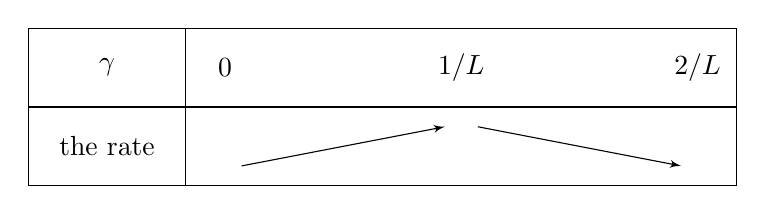
\begin{tikzpicture}
                \tkzTabInit{$\gamma $ / 1, the rate / 1}{ $0$, $1/L$, $2/L$ }
                \tkzTabVar{ -/, +/, -/}
             \end{tikzpicture}
            \item Optimal "constant" step size $ = \frac{1}{L} $ 
        \end{enumerate}
    \end{note}

    \begin{note}[Interpolation of GD with $ \gamma = \frac{1}{L} $ ]
        Note that \begin{align*}
            \tilde{\theta }_t 
                &= \arg \min F(\tilde{\theta }_{t-1}) + \langle \nabla F(\tilde{\theta } _{t-1}), \theta  - \tilde{\theta }_{t-1} \rangle + \frac{L}{2} \left\| \theta  - \tilde{\theta }_{t - 1} \right\| ^2 \\
                &= \tilde{\theta }_{t - 1} - \frac{1}{L} \nabla F(\tilde{\theta }_{t - 1})
        \end{align*}
        Using GD with $ \gamma = \frac{1}{L} $ amounts to minimizer a quadratic upper bound (provided by smoothness). This idea is a the heart of the Majorize-Minimize algo. 
    \end{note}
\end{thm}

\begin{proof}[Proof:]
    \begin{align*}
        \left\| \theta _{t+1} - \theta ^\star  \right\| ^2 _2  
            &= ^{\text{(GD)}} \left\| \theta _t - \gamma \nabla F(\theta _t) - \theta ^\star  \right\| ^2 _2 \\
            &= \left\| \theta _t - \theta ^\star  \right\| ^2 _2 - 2 \gamma  \langle \nabla F(\theta _t), \theta _t - \theta ^\star \rangle + \gamma ^2 \left\| \nabla F(\theta _t) \right\| ^2 _2
    \end{align*}
    Function convex + L-Smooth : $ \left\| \nabla F(\theta ) \right\| ^2 \leq L \langle \nabla F(\theta ), \theta  - \theta ^\star \rangle $. This is a consequence of the co-coercivity of $ \nabla F $ (with param $ 1/L $ )
    \begin{note}[Co-coercivity]
        $ F $ convex, L-Smooth, then $ \theta , \theta ^\prime  $ 
        \[
            \langle  \nabla F(\theta ) - \nabla F(\theta ^\prime ), \theta  - \theta ^\prime \rangle \geq_{\text{co-coercivity}} \frac{1}{L} \left\| \nabla F(\theta ) - \nabla F(\theta ^\prime ) \right\| ^2 _2
        .\]
        \begin{proof}[Proof of the note on co-coercivity:]
            Define two function \begin{align*}
                G(\theta ^\prime ) &= F(\theta ^\prime ) - \langle \nabla F(\theta ) , \theta ^\prime \rangle  \\
                H(\theta ^\prime ) &= F(\theta ) - \langle \nabla F(\theta ^\prime ), \theta \rangle 
            \end{align*}
            $ G $ and $ H $ are smooth. $ \theta ^\prime = \theta  $ minimize $ \theta ^\prime  \mapsto G(\theta ^\prime ) $ and 
            \begin{align*}
                F(\theta ^\prime) - F(\theta ) - \langle \nabla F(\theta ) , \theta ^\prime - \theta  \rangle
                    &= G(\theta ^\prime) - G(\theta ) \\
                    &\geq \frac{1}{2L} \left\| \nabla G(\theta ^\prime ) \right\| ^2 (\text{by LHS, 1) and where "all in all"} ) \\
                    &= \frac{1}{2L} \left\| \nabla F(\theta ^\prime ) - \nabla F(\theta ) \right\| ^2
            \end{align*} 
            Idem, $ \theta  = \theta ^\prime  $ minimizes $ \theta \mapsto H(\theta ) $ 
            \begin{align*}
                F(\theta ) - F(\theta ^\prime ) - \langle \nabla F(\theta ^\prime ), \theta  - \theta ^\prime \rangle &= H (\theta ) - H(\theta ^\prime ) \\
                &\geq \frac{1}{2L} \left\| \nabla H(\theta )  \right\| ^2 \\
                &= \frac{1}{2L} \left\| \nabla F(\theta ^\prime ) - \nabla F(\theta ) \right\| ^2
            \end{align*}
            Sum the 2 inequalities to conclude
        \end{proof}
        End of the co-coercivity note
    \end{note}
    
    \begin{align*}
        \left\| \theta _{t+1} - \theta ^\star  \right\| ^2 
            &= \left\| \theta _t - \theta ^\star  \right\| ^2 - 2 \gamma  \langle \nabla F(\theta _t), \theta _t - \theta ^\star \rangle + \gamma  ^2 \left\| \nabla F(\theta _t) \right\| ^2 \\
            &\leq  \left\| \theta _t - \theta ^\star  \right\| ^2 - 2 \gamma ( 1 - \frac{\gamma L }{2}) \langle \nabla F(\theta _t) , \theta _t - \theta ^\star \rangle  \\
            &\Rightarrow 2 \gamma (1 - \frac{\gamma L}{2}) \langle \nabla F(\theta _t) , \theta _t - \theta ^\star \rangle \leq  \left\| \theta _{t-1} - \theta ^\star  \right\| ^2 - \left\| \theta _t - \theta ^\star  \right\| ^2  \\
            &\Rightarrow 2 \gamma (1 - \frac{\gamma L }{2}) (F(\theta _t) - F(\theta ^\star )) \leq  \left\| \theta _{t-1} - \theta ^\star  \right\| ^2 - \left\| \theta _t - \theta ^\star  \right\| ^2  \\
            &\Rightarrow F(\theta _t) - F(\theta ^\star )
            \leq \frac{1}{T}\sum_{t=1}^{T} F(\theta _t) - F(\theta ^\star ) \\
            &\leq \frac{\left\| \theta _0 - \theta ^\star  \right\| ^2}{ 2 \gamma (1 - \frac{\gamma L}{2}) T}
    \end{align*}
    
\end{proof}

\underline{Nouveau cours du 23/11} \\


RAPPEL : 
On regarde \begin{itemize}
    \item $ \theta _{t+1} = \theta _t - \gamma _t \nabla F(\theta _t)$ 
    \item $ \theta _0 \in \mathbb{R}^d $ 
\end{itemize}

\begin{thm}[]
    F L-smooth, diff \\
    For $\gamma_t = \gamma$ for all $t \leq0$
    
    \begin{align*}
        F(\theta _T) - F(\theta ^\infty ) 
            &\leq \frac{\left\| \theta _0 - \theta ^\infty \right\| ^2}{2 \gamma (1 - \frac{\gamma L}{2} )T} \\
            &= L \frac{\left\| \theta _0 - \theta ^\infty  \right\| ^2 }{T} (\gamma = 1/L)
    \end{align*}


    \begin{itemize}
        \item $\gamma = \dfrac{1}{L}$ It is the largest constant step size ensuring the most decrease of the objective fct at each iteration.
        \item L-smooth, diff $\mathcal{C}^2 \Leftrightarrow \lambda_{MAX}(H_F(\theta)) \leq L \forall \theta $
        \begin{align*}
            \Leftarrow  \left\| \nabla F(\theta ) - \nabla F(\theta ^\prime ) \right\|  
                &= \left\| \int_{0}^{1} H_F (\theta ^\prime + t ( \theta  - \theta ^\prime )) (\theta  - \theta ^\prime ) dt \right\| \\
                &\leq \int_{0}^{1} \left\| H_F (\theta  + t (\theta  - \theta ^\prime )) (\theta  - \theta ^\prime ) \right\| dt \\
                &\leq L \left\| \theta - \theta ^\prime  \right\| _2
        \end{align*}
    \end{itemize}
\end{thm}

\begin{thm}[]
    If $ F $ is L-Smooth, diff and $ \mu  $ - strongly convex, then for all step size $ \gamma \leq 1/L $ 
    \begin{align*}
        \left\| \theta _T - \theta ^\star  \right\| ^2 
            &\leq (1 - \gamma \mu ) ^T \left\| \theta _0 - \theta ^\star  \right\| ^2 \\
            (\text{for } \gamma = 1/L) &= (1 - \frac{\mu }{L}) ^T \left\| \theta _0 - \theta ^\star  \right\| ^2 (\text{for } \gamma = 1/L)
    \end{align*}
\end{thm}

\begin{note}
    \begin{enumerate}
        \item The algorithm is the same so the CV rate is improved only by properties of F. In such a case the rate is said to be linear.
        \item CV rate on the iterates (!!) and not only on the objective rate 
        \begin{align*}
            F(\theta _T) - F(\theta ^\star ) 
            &\leq \langle \nabla F(\theta ^\infty ), \theta _T - \theta  ^\star \rangle  + \frac{L}{2} \left\| \theta _T  - \theta ^\star \right\| \\
            &= 0 + \frac{L}{2} \left\| \theta _T  - \theta ^\star \right\|
        \end{align*}
        
        \[
            \frac{\mu }{2} \left\| \theta _T - \theta ^\star  \right\| ^2 \leq_{\text{strong cvxty}}  F(\theta _T) - F(\theta ^\star ) \leq  + \frac{L}{2} \left\| \theta _T  - \theta ^\star \right\|
        .\]
        \item Choice of $\gamma$ : the largest possible.
        \item $\mu \leq L$. ($\mu = L$ if $F(\theta)= \dfrac{L}{2}\left\| \theta - \theta ^ {\star} \right\| $)
    \end{enumerate}

    So : \begin{itemize}
        \item $\kappa = \dfrac{\mu}{L}$ is called the condition number of F.
        \item $\kappa << 1$ "Bad conditioning"
        \item $\kappa \simeq 1$ "good conditioning"
    \end{itemize}

    \begin{figure}[!htbp]
        \centering
        \includegraphics[width=.5\textwidth]{figs/bad_kappa.jpg}
        \caption{With $ \kappa \ll 1 $ "bad conditioning" }
    \end{figure}
    
    \begin{figure}[!htbp]
        \centering
        \includegraphics[width=.5\textwidth]{figs/good_kappa.jpg}
        \caption{With $ \kappa \approx 1 $ "good conditioning" }
    \end{figure}

    \begin{proof}[Proof:]
        \begin{align*}
            \left\| \theta _{t+1} - \theta ^\star  \right\| ^2 
                &= \left\| \theta _t - \gamma \nabla F(\theta _t) - \theta ^\star  \right\| ^2 \\
                &= \left\| \theta _t - \theta ^\star  \right\| ^2 - 2 \gamma \left\langle \nabla F (\theta _t), \theta _t - \theta ^\star  \right\rangle + \gamma ^2 \left\| \nabla F(\theta _t) \right\| ^2 \\
                &= \left\| \theta _t - \theta ^\star  \right\| ^2 - 2 \gamma \left\langle \nabla F (\theta _t), \theta ^\star - \theta _t \right\rangle + \gamma ^2 \left\| \nabla F(\theta _t) \right\| ^2 \\
        \end{align*}
        By $ \mu  $-strong convexity, we got 
        \begin{align*}
            &F(\theta ^\star ) \geq F(\theta _t) + \left\langle \nabla F(\theta _t) , \theta ^\star - \theta _t  \right\rangle + \frac{\mu }{2}\left\| \theta ^\star - \theta _t \right\| ^2 \\
            & \Rightarrow \left\langle \nabla F(\theta _t) , \theta ^\star - \theta _t \right\rangle \leq F(\theta ^\star ) - F(\theta _t) - \frac{\mu }{2}\left\| \theta ^\star -  \theta _t \right\| ^2
        \end{align*}
        
        Therefore $\left\| \theta_{t+1} - \theta^{\star }  \right\|^2 \leq \left\| \theta_t - \theta^{\star }\right\|^2 - 2 \gamma (F(\theta_t) - F(\theta ^{\star }) + \dfrac{\mu}{2} \left\| \theta ^{\star } - \theta_t \right\|^2 ) + \gamma ^2 \left\| \nabla F(\theta_t ) \right\|^2    $

        Beside, by L-smoothness, we get 
        \begin{align*}
            F(\theta _{t+1}) - F(\theta _t) 
                &= F(\theta _t - \gamma \nabla F(\theta _t)) - F(\theta _t) \\
                &= [F(\theta _t - \tau \nabla F(\theta _t))]^\gamma _{\tau = 0} \\
                &= -\int_{0}^{\gamma } \left\langle \nabla F(\theta _t), \nabla F(\theta _t - \tau \nabla F(\theta _t)) \right\rangle d \tau \\
                &= -\int_{0}^{\gamma } \left\langle \nabla F(\theta _t), \nabla F(\theta _t - \tau \nabla F(\theta _t)) \right\rangle + \nabla F(\theta _t) - \nabla F(\theta _t) d \tau \\
                &= - \gamma \left\| \nabla F(\theta _t) \right\| ^2 + \int_{0}^{\gamma } \left\langle \nabla F(\theta _t), \nabla F(\theta _t) - \nabla F(\theta _t - \tau \nabla F(\theta _t)) \right\rangle d \tau \\
                &\leq - \gamma \left\| \nabla F(\theta _t)  \right\| ^2 + \int_{0}^{\gamma }\tau L \left\| \nabla F(\theta _t) \right\| ^2 d \tau  \\
                &\leq - (\gamma - \frac{\gamma ^2 L}{2}) \left\| \nabla (F(\theta _t )) \right\| ^2 \text{ using CS + L-smooth}
        \end{align*}
        Combining the 2 previous inequalities, 
        \begin{align*}
            \left\| \theta_{t+1} - \theta ^{\star} \right\|^2 &\leq  \left\| \theta_{t} - \theta ^{\star} \right\|^2 (1 - \gamma \mu ) - 2 \gamma (F(\theta_t) - F^{\star }) + \frac{\gamma ^2 }{\gamma - \gamma^2 \frac{L}{2}} \\
            &\leq (1 - \gamma \mu ) \left\| \theta_t - \theta ^\star  \right\| ^2 - \gamma ( \frac{2 \gamma - \gamma ^2 \frac{L}{2} - \gamma }{\gamma - \gamma ^2 \frac{L}{2}}) ( F(\theta _t ) - F^\star )
        \end{align*}
        using that $ F(\theta ) \geq F(\theta ^\star ) \Rightarrow F(\theta _t) - F(\theta _{t+1}) \leq F(\theta _t) - F(\theta ^\star ) $  
        \begin{itemize}
            \item Numerator $ > 0 $  when $ 0 < \gamma \leq 1/L $ 
            \item Denominator $ > 0 $  when $ 0 < \gamma < 2/L $ 
        \end{itemize}
        Then by assuming $ \gamma \leq \frac{1}{L} $ just ignore the last term and conclude
    \end{proof}
\end{note}



\subsubsection{Subgradient method}
\begin{thm}[GD for non-smooth fonctions]
    Hypothese : $ F $ convex, has subgradients, $ \beta  $ -Lipschitz 
        \[
            \begin{cases}
                \left\| \nabla F(\theta ) \right\| ^2 &\leq \beta ^2\\
                \left\| \eta  \right\| ^2 &\leq \beta ^2, \quad \forall \eta \in \partial F(\theta)
            \end{cases} 
        .\]
    Then GD iterates with Polyak-Ruppert averaging enjoy the following error bound 
    
    \[
        \bar{\theta }_T = \frac{1}{T} \sum_{t=1}^{T} \theta _t
    .\]
    
    \begin{align*}
        F(\bar{\theta_T}) - F(\theta ^{\star}) 
            &\leq \frac{\left\| \theta_0 - \theta ^{\star } \right\|^2 }{2 \gamma T} +  \frac{\gamma \beta ^2}{2} \\
            &= \textcolor{orange}{\left\| \frac{\theta _0 - \theta^{\star }}{\sqrt[]{T}} \right\| \text{ for } \gamma = \gamma ^{\star}} 
        \text{ (when looking at below figures)}
    \end{align*}
    \[
        F(\bar{\theta_T}) - F(\theta ^{\star}) \leq \frac{\left\| \theta_0 - \theta ^{\star } \right\|^2 }{2 \gamma T} +  \frac{\gamma \beta ^2}{2}     
    .\]
\end{thm}
NB: now there is a trade-off on the choice of $ \gamma  $. Now we have two terms : 
\begin{itemize}
    \item $ \frac{\left\| \theta_0 - \theta ^{\star } \right\|^2 }{2 \gamma T}  $ in purple in Figure \ref*{fig:tradeoff}
    \item $ \frac{\gamma \beta ^2}{2}  $ in green  in Figure \ref*{fig:tradeoff}
\end{itemize}
\begin{figure}[!h]
    \centering
    \includegraphics[width=.75\textwidth]{figs/gamma_compromise.jpg}
    \caption{ }
    \label{fig:tradeoff}
\end{figure}
One can choose $ \gamma ^\star  $ such that "purple" = "green" (Figre \ref*{fig:tradeoff}), i.e. 
\[
    (\gamma ^\star )^2 = \frac{\left\| \theta _0 - \theta ^\star  \right\| ^2}{\beta ^2 T}
.\]

\begin{itemize}
    \item Non-smoothness is paid through a $ O(\frac{1}{\sqrt[]{T}}) $ rate. 
    
    \item Guarantee for $ \bar{\theta} _T $ 
    
    \item CCL Big picture : BD-Based strategies 
    \begin{itemize}
        \item convex non-smooth $ O(1 / \sqrt[]{T}) $ 
        \item convex L-smooth $ O(1 / T) $ 
        \item $ mu $-strongly convex non-smooth $ O( ( 1 - \frac{\mu }{L})^T ) $ 
    \end{itemize}
\end{itemize}
$F(\frac{1}{T} \sum^T_{t=1} \theta_t) - F^{\star } \leq \frac{1}{T} \sum^T_{t=1} (F(\theta _t) - F^{\star })$ by convexity. \\
And $(F(\theta _t) - F^{\star })$ is on $\frac{1}{t}$ \\
So, $F(\frac{1}{T} \sum^T_{t=1} \theta_t) - F^{\star } \leq \frac{1}{T} \sum^T_{t=1} (F(\theta _t) - F^{\star }) \lesssim \mathcal{O}(\frac{\log_{T}}{T})$.

\begin{proof}[Proof:]
    \begin{align*}
        \left\| \theta _{t + 1} - \theta ^\star  \right\| ^2 
            &= \left\| \theta _t - \gamma _t g_t - \theta ^\star  \right\| ^2 \text{ with } g_t \in \partial F(\theta _t) \\
            &= \left\| \theta _t - \theta ^\star  \right\| ^2 - 2 \gamma _t \left\langle g_t , \theta _t - \theta ^\star \right\rangle + \gamma _t ^2 \left\| g_t \right\| _2 ^2 \\
            \text{by def of subgradient } &\leq \left\| \theta _t - \theta ^\star  \right\| ^2 - 2 \gamma _t (F(\theta _t) - F^\star ) + \gamma _t ^2 \left\| g_t \right\| _2 ^2 
    \end{align*}
    Recursively we obtain 
    \[
        \left\| \theta _{t+1} - \theta ^\star  \right\| ^2 \leq  \left\| \theta _1 - \theta ^\star  \right\| ^2 - 2 \sum_{s=1}^{t} \gamma _s (F(\theta _s) - F^\star ) + \sum_{s=1}^{t} \gamma _s ^2 \left\| g_s \right\| _2 ^2 
    .\]
    
    Combining this with $\sum_{s=1}^t \gamma _s (F(\theta _s) - F^{\star }) \geq \sum_{s=1}^t \gamma_s. \min_{1 \leq s \leq t} (F(\theta _s) - F^{\star })$ \\
    $\gamma$ cte + polyak- Ruppert \\
    $t \sum_{s=1}^t \frac{\gamma_s}{t}(F(\theta _s) - F^{\star }) \geq t \gamma (F(\bar{\theta _t}) - F^{\star })$ 


    Finally, 
    \begin{align*}
        \min _{1 \leq s \leq t} F (\theta _s) - F^\star 
        &\leq \frac{\left\| \theta _1 - \theta ^\star  \right\|_2 ^2 + \sum_{s=1}^{t} \gamma _s \left\| g_s \right\|_2 ^2  }{2 \sum_{s=1}^{t} \gamma _s} \\
        &\leq \frac{\left\| \theta _1 - \theta ^\star  \right\|_2 ^2 + \beta ^2 \sum_{s=1}^{t} \gamma _s  }{2 \sum_{s=1}^{t} \gamma _s} \\
        F(\bar{\theta}_t) - F^\star &\leq \frac{\left\| \theta _1 - \theta ^\star  \right\| ^2 + t \gamma ^2 \beta ^2}{2t \gamma}
    \end{align*}
\end{proof}

\begin{note}[Implicit gradient method]
    Subgradient method = generalization of GD in the non-smooth case but $ O $ is typically slow ($ \frac{1}{\sqrt[]{T}} $ ). 

    The essential reason is that there are plenty of subgradients that are large near and event at the solution.

    $ g \in \partial F(\theta ) $ if $ \forall \theta ^\prime, F(\theta ^\prime ) \geq F(\theta ) +  \left\langle g, \theta ^\prime - \theta  \right\rangle $ 
    \[
        \partial ? (\theta ) = \begin{cases}
            \{ +1 \}  &\text{ if } \theta > 0\\
            \{ -1 \}  &\text{ if } \theta < 0\\
            [-1 , 1]  &\text{ if } \theta = 0\\
        \end{cases} 
    .\]
    
    \begin{figure}[!h]
        \centering
        \includegraphics[width=.65\textwidth]{figs/subgradients.jpg}
        \caption{sub gradiens}
        \label{truc}
    \end{figure}

    Another way to deal with this is to add a smooth regularized term. In particular, if $\theta ^{\star }$ is minimizer of F then it minimizes as well
    \[ \theta  \mapsto F(\theta) + \gamma \left\| \theta - \theta ^{\star } \right\| \text{ for } \gamma > 0  \]

    Now the regulatized fonction is strongly convex and the only subgradient at the solution is the zero vector : \begin{itemize}
        \item \textbf{Good} : It addresses the main drawback of subgrad methods
        \item \textbf{Bad} : We have to know $ \theta ^\star  $ 
    \end{itemize}

    One can implement an iterative version of it, this is the proximal algo : 
    \[ 
        \theta _{t+1} = \arg \min_{\theta} F(\theta) + \frac{1}{2 \gamma _t} \left\| \theta - \theta_t  \right\|^2 
    \]
    When $ F $ is convex, $ F + \frac{1}{2 \gamma _t} \left\| \circ  - \theta _t \right\| ^2 $ is strictly convex so the mapping is well defined. This gives the proximal operator / Moreau envelope. 
    
    \[
        prox _{\gamma _t F} (\theta ) = \arg \min_{\tilde{\theta}} F(\tilde{\theta }) + \frac{1}{2 \gamma _t} \left\| \theta - \tilde{\theta}  \right\|^2 
    .\]

    The proximal operator can be interpreted as a variation of gradient methods 
    
    \[
        \begin{cases}
            \frac{d \theta }{dt}(t) = - \nabla F(\theta ) \\
            \theta (0) = \theta _0 \in \mathbb{R}^d
        \end{cases}
    .\]
    The equilibrium points of this system are the $\theta $'s such that $\nabla F(\theta )= 0$, i.e the minimizers of $ F $  when $ F $  is convex
    
    GD = 1st order numerical method for tracing the path from $ \theta _0 $ to $ \theta ^\star  $ 
    \[
        \frac{\theta (t + h) - \theta (t)}{h} \approx - \nabla F(\theta (t))
    .\]
    
    GD $\equiv$ Forward Euler discretization. \\
    But we could use Backward instead 
        
    \[
        \frac{\theta (t) - \theta (t -h)}{h} \approx - \nabla F(\theta (t))
    .\]
    And now the iterates obey :
    \[
        \theta_{t+1} = \theta _t - h \nabla F(\theta_{t+1}) \qquad \text{"Implicit"}
    .\]
    Their construction is not straight forward anymore. But this is what the prox operator actually computes 
    \begin{align*}
        \theta _{t+1} = \arg \min F(\theta _t) + \frac{1}{\gamma _t } \left\| \theta -\theta _t \right\| ^2 \\
        \Leftrightarrow 0 = \nabla F(\theta _{t + 1}) + \frac{1 }{\gamma _t} (\theta _{t+1} - \theta _t)
    \end{align*}
\end{note}


\begin{note}[Newton's method]
    Given $ \theta _{t-1} $, the Newtons's method minimizes the 2nd ordre Taylor expansion arount $ \theta _{t-1} $ 
    \[
        \theta \mapsto F(\theta_{t-1}) + \left\langle \nabla F(\theta _{t-1}, \theta  - \theta _{t-1}) \right\rangle + \frac{1}{2} (\theta  - \theta _{t-1} )^T Hess_F(\theta _{t-1}) (\theta - \theta _{t-1})
    .\]
    the gradient of this quadratic form is 
    \[
        \nabla F(\theta _{t-1}) + H_F(\theta _{t-1})^{-1} \nabla F(\theta _{t-1})
    .\]
    Exercise : Check that $- H_F(\theta_{t-1})^{-1} \nabla F(\theta_{t-1})$ is indeed a descent direction of F at $\theta_{t-1}$.
    
    Newton's method are methods of order 2 : using the gradient (order 1) and the Hessian (order 2). Running-time complexity is $ O(d^3) $ in general to solve the linear system. 

    It leads to local quadratic CV : 
    \[
        (C \left\| \theta_t - \theta ^{\star}\right\| ) \leq (C \left\| \theta_t - \theta ^{\star}\right\| )^2
    .\]
    For global convergence guarantees, see  \textit{Boyd \& Vandenberghe (2004)} in particular using the self-concordance relating 3rd and 2nd order derivatives. 
\end{note}

\section{Inertial methods}

\subsection{Préliminaries}
So far we have \begin{itemize}
    \item convex, L-smooth : $ O(1/k) $ 
    \item strongly convex, L-smooth : $ O((1 - \frac{\mu }{L}) ^k ) $ 
\end{itemize}

Can we do better with a \textbf{gradient-like} algo ? 

\begin{defn}[]
    A gradient-like algo is an algo such taht 
    \[
        \theta _{t+1} \in span \{\theta _0, \dots, \theta _t, \nabla F(\theta _0), \dots, \nabla F(\theta _t)\}
    .\]
\end{defn}

\begin{thm}[Nemirovski-Rudin 1983]
    $\forall \theta_0 \in \mathbb{R}^d, \forall 0 \leq t \leq \frac{d-1}{2}$ \\
    $ \exists F $  convex, L-smooth such that for every gradient-like algon we have 
    \[
        F(\theta _t) - \inf F \geq \frac{3L \left\| \theta ^0 - \theta ^\infty  \right\| }{32 \mathbf{(t + 1)^2}}
    .\]
\end{thm}

\begin{thm}[Nesterov 2003]
    $ \forall \theta _0 \in \mathbb{R}^d, \mu > 0, L > 0, \exists F $ $ mu $-strongly convex and L-smooth such that for every gradient-like algo \begin{enumerate}
        \item $ F(\theta _t) - \inf F \geq  \frac{\mu }{2} ( \frac{1 - \sqrt[]{\kappa }}{1 + \sqrt[]{\kappa }} )^{2t} \left\| \theta _0 - \theta ^\star  \right\|  $ 
        \item $\left\| \theta _t - \theta ^{\star } \right\| \geq (\frac{1 - \sqrt[]{\kappa }}{1 + \sqrt[]{\kappa }})^t \left\|  \right\| \theta _0 - \theta ^{\star } \quad $ with $\kappa = \frac{\mu }{L}$ 
    \end{enumerate}
\end{thm}

Can we design first-order strategies that achieve convergence rates matching these lower bounds ? 

\subsection{Heavy ball dynamics}

\[
    \ddot{\theta }(t) = - \alpha (t) \dot{\theta } - \nabla F(\theta (t)), (\alpha (t) > 0 )
.\]
We add a function term to the gradient flow. 

We can have a look at the quantity 
\[
    \epsilon (t) = F(\theta (t)) - \inf F + \frac{1}{2} \left\| \dot{\theta }(t) \right\| ^2 = E_{pot} + E_{cin}
.\]

We can show that $ \epsilon (t) $ is decreasing (this is a Lyapunov energy) 
\begin{align*}
    \dot{\epsilon }(t) \\
        &= \left\langle \nabla F(\theta (t)) , \dot{\theta }(t) \right\rangle + \left\langle \ddot{\theta }(t) , \dot{\theta }(t) \right\rangle \\
        &= \left\langle \ddot{\theta }(t) + \nabla F(\theta (t)), \dot{\theta }(t) \right\rangle \\
        &= - \alpha (t) \left\| \dot{\theta }(t) \right\| ^2 \mathbf{()\leq 0)}
\end{align*}

\begin{note}
    $ \alpha (t) \equiv 0 $  gives a conservative dynamics with aliittle hope of CV.

    \begin{align*}
        F(\theta ) &= \frac{1}{2}\theta ^2, \alpha = 0 \\
        \ddot{\theta }(t) &= - \theta (t) \Leftrightarrow \theta (t) = c_1 \sin (t) + c_2 \cos (t)
    \end{align*}
    Why it can help? Gabriel Goh "Why momentum really works".
    \[
        \ddot{\theta }(t) = - \alpha (t) \dot{\theta }(t) - \nabla F(\theta (t))
    .\]
    
    \paragraph*{Discretization }
    \begin{align*}
        \theta (t_k) & \approx \theta _k \\
        \dot{\theta } (t_k) & \approx \frac{\theta _k - \theta _{k-1}}{h} \\
        \ddot{\theta } (t_k) & \approx \frac{\dot{\theta }(t_{k+1}) - \dot{\theta }(t_k)}{h} \\
        \frac{\theta _{k+1} - 2 \theta _{k} + \theta _{k+1}}{h^2} + \alpha (t_k) \frac{\theta _{k}- \theta _{k-1} }{h} &+ \nabla F(\theta _{k}) = 0
    \end{align*}
    
    Define $\gamma = h^2$  $\alpha_k = \frac{\alpha (t_k)}{\sqrt[]{\gamma }}$ we get :
    \[
        \theta _{k+1} = \theta _{k} - \gamma \nabla F(\theta _{k}) + (1 - \alpha_k )(\theta _{k} - \theta _{k-1})
    .\]
    where $\gamma \nabla F(\theta _{k})$ is the gradient step and \\
    $ (1 - \alpha_k )(\theta _{k} - \theta _{k-1})$ is the inertia : memory of the last iterates. [polyak 64]


    \paragraph*{HEAVYBALL}[Polyak, 64]
    \begin{align*}
        \beta _k &= \theta _k + (1 - \alpha _k) (\theta _k - \theta _{k-1}) \\
        \theta _{k+1} &= \beta _k - \gamma \nabla F(\theta _k)
    \end{align*}

    \paragraph*{NESTEROV ALGO}[83]
    \begin{align*}
        \beta _k &= \theta _k + (1 - \alpha _k) (\theta _k - \theta _{k-1}) \\
        \theta _{k+1} &= \beta _k - \gamma \nabla F(\beta _k)
    \end{align*}

    They look the same, the only difference is where the gradient is evaluated. Both algo come with 2 choices for the friction $ \alpha _k $ \begin{itemize}
        \item constant friction $ \alpha _k \equiv \alpha \sqrt[]{\gamma } $ (for good functions)
        \item vanishing friction  $ \alpha _k \equiv \frac{\alpha}{k}  $ (for bad functions)
    \end{itemize}
\end{note}

\paragraph*{HEAVY BALL}
\begin{thm}[polyak 64, écrit vite fait parce que c'est la fin du cours]
    F quadratic -smooth, m$\mu$- strongly cvx, $\kappa = \frac{\mu }{L}$ with,

    \[
        \begin{cases}
            \gamma = \frac{4}{L(1+K)^2} \\
             \alpha _k = \frac{2 \sqrt[]{\mu } \gamma }{1 + \sqrt[]{\kappa }}
        \end{cases} 
    .\]
    CV rate $\mathcal{O}((\frac{1 - \kappa }{1 + \kappa })^t )$

    Cool : We have Optimal rate and constant friction is enough \\
    But : HB can fail on general strongly convex fonction and need to know $ \mu  $  (and $ L $ )
\end{thm}

\paragraph*{NESTEROV}
\begin{thm}[]
    F L-smooth, $\mu$-strongly cvx
    Choose $ \gamma  = 1/L, \alpha = \frac{\sqrt[]{L} - \sqrt[]{\mu }}{ \sqrt[]{L} + \sqrt[]{\mu }} $ to get $ (1 - \sqrt[]{\frac{\mu }{L}}) $ -linear CV (convergence)

    Cool : Better GD \\
    Questionnable : Not optimal
\end{thm}

\begin{thm}[Nesterov 83, Chambolle-Dossal 2015]
    F convex, L-smooth
    $ \gamma \leq 1/L, \alpha _k = \alpha / k $ with $ \alpha \geq 3 $ 
    \[
        F(\theta _k) - F^\star \leq O(\frac{1}{k^2})
    .\]
    
    Cool : Optimal
\end{thm}

We can take other choices for decreasing $(\alpha _k)_k$, the historical choice is


\[
    \text(Friction : )(1 - \alpha _k) = \frac{t_k - 1 }{t_{k+1}} \text{ with } \begin{cases}
        t_1 = 1 \\
        t_{k+1} = \frac{1 + \sqrt[]{1 + 4 t _k ^2}}{2} \\
    \end{cases} 
.\]
CCL : Essayer les deux méthodes : speed upped or not 

\begin{figure}[htbp]
    \centering
    \includegraphics[width=.95\textwidth]{figs/table_conv_speed.jpg}
    \caption{Tableau de la vitesse de convergence des algos}
\end{figure}

CCL : vanishing friction helps on the worst fcts


\end{document}